\chapter{Tashlhiyt, a Berber language}
\section{The Imazighen}
The Imazighen (Amazighs, Berbers) are the native inhabitants of wide parts of North Africa extending from the coast of the Atlantic Ocean to the Siwa oasis in Egypt. The language spoken by the Imazighen is henceforth referred to as "Berber" (it is also referred to as "Tamazight").\footnote{In the following, the languages spoken by the Imazighen are referred to as "Berber". This term is used as a neutral term and has no negative connotation in an Anglo-Saxon context. While the term "Tamazight" has become popular among modern Berber intellectuals, we refrain from using the term here because of its ambiguity: Tamazight can be used to refer either to the Berber language as denoting the language family in general or to the specific Berber variety spoken in central Morocco (as opposed to Tashlhiyt in the South).} Berber has been classified as belonging to the Afro-Asiatic language family, which also includes Ancient Egyptian, Chadic, Cushitic, Omotic, and Semitic languages (\citealt{Ethnologue2016}). For a general overview of the language family see \citet{Basset1952}, \citet{Applegate1971} and \citet{Galand1988}.

Berber is spoken by a substantial number of people in Algeria, Tunisia, Libya, Egypt, Mauritania, Burkina-Faso, Mali, and Niger with the majority of speakers living in Morocco. Moroccans are often native speakers of one or more Berber languages alongside a Moroccan variety of Arabic. The long-lasting language contact between Moroccan Arabic and Berber is reflected in highly overlapping vocabularies, a result of massive borrowing in Berber (\citealt{Kossmann2009}).

Morocco is described as having three major Berber languages: "Tarifiyt" \il{Berber (Tarifiyt)} spoken in the north, "Tamazight" \il{Berber (Tamazight)} spoken in the Middle Atlas region and "Tashlhiyt",\footnote{Alternatively, the language or specific subvarieties of it have been referred to as Shilha and Soussiya (Susiya, Tasoussit). Tashlhiyt has also been spelled Tachilhit, Tashelhaït, Tashelhit or Tashilheet.} the variety under investigation here, spoken in the High-Atlas region and south of it (\figref{fig:3.1}). While there is a clear geographic separation of Tarifiyt and the southern varieties reflected in a clear-cut linguistic distinction, the distinction between Tamazight and Tashlhiyt is better captured by a continuum. The number of Tashlhiyt speakers is unclear. Estimates range from three million (\citealt{Chaker1992}) to 3.9 million speakers in 2004 (\citealt{Ethnologue2016}), with Berber in general being currently spoken by about 7.7 million people in Morocco  (\citealt{Ethnologue2016}). These numbers may diverge so drastically due to the historically loaded multilingual context in Morocco, which will be sketched briefly below.


\begin{figure}
   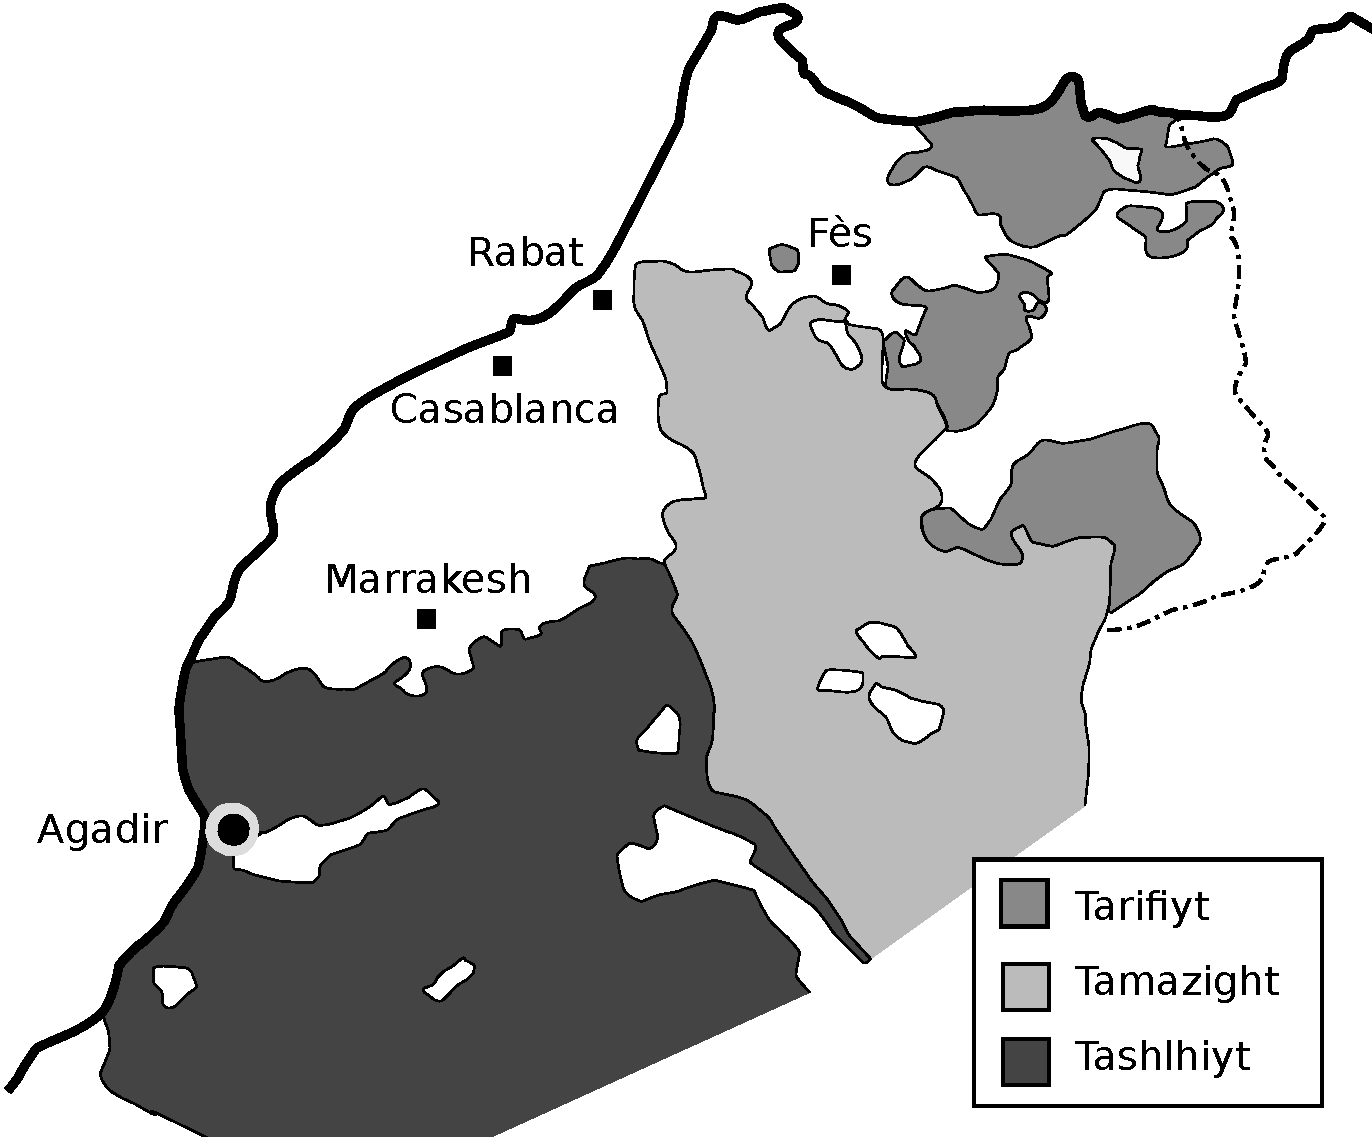
\includegraphics[width=0.9\textwidth]{figures/Figure_3_1.pdf}
  \caption{Map of the three major Berber languages spoken in Morocco alongside the location of major cities. The large circle indicates the location of Agadir, the city in which the Tashlhiyt variety investigated here is spoken. White spaces indicate non-Berber speech communities. This map is based on the map by \citet[203]{colin1937}.}
   \label{fig:3.1}
   \end{figure}

In addition to at least one Berber variety, Moroccans are often speakers of Moroccan Arabic. In some areas, speakers may additionally have a high degree of proficiency in French, a residual of the French colonisation. It is clear that this intricate multilingual situation in Morocco plays an important role in any evaluation of the linguistic structures of Moroccan languages. Therefore, a brief historical overview of the Imazighen in North Africa and the history of Morocco is given below (\sectref{sec:3.2}). The linguistic description presented in this book is based on recordings of university students from Agadir. We will briefly discuss relevant facts about Agadir and the speaker sample (\sectref{sec:3.3}). Subsequently, we will give a succinct overview of the linguistic system of Tashlhiyt (\sectref{sec:3.4}). This will include an introduction to the orthographic systems used by Tashlhiyt speakers (\sectref{sec:3.4.1}), a presentation of the phoneme inventory of the language, relevant phonetic properties of phonological contrasts, and relevant aspects of syllable structure (\sectref{sec:3.4.2}), a presentation of basic morphological patterns (\sectref{sec:3.4.3}), and a description of basic word order and syntactic constructions (\sectref{sec:3.4.4}).

\section{Historical overview}\label{sec:3.2}
The Imazighen were the first inhabitants of North Africa, as testified by historical, anthropological, archaeological, and linguistic records (e.g. \citealt{Julien1966,Laroui2015}). The first Imazighen in Morocco were farmers and merchants trading with people from the Mediterranean early on. Over the centuries, they were heavily influenced by other civilisations such as the Phoenicians, the Carthaginians, the Romans, and the Vandals, all of which left a lasting effect on their religious belief, arts, and language. However, no civilisation had a greater impact on the Imazighen than the Arab civilisation. The Arabs arrived in Morocco in 682 CE. As the Berbers had no significant literary tradition, the Arabic language spread quickly and manifested itself as the language of science, administration, and, of course, the language of the Qur’an.
 

Another linguistically significant historical event was the French Protectorate. At the beginning of the 20th century, France established a protectorate over Morocco. The French Protectorate lasted from 1912 to 1956 and had, yet again, a huge impact on political, educational, and economic aspects of the country. The French introduced new educational systems, which, crucially, distinguished between a very constrained Islamic system and an Imazighen system that did not contain Islamic studies. Both Arab and Imazighen communities protested. It was perceived as an attack on Moroccans' cultural and religious identity since the education in Classical Arabic was a crucial aspect of religious practice (\citealt{Zouhir2013}). Later, in 1930, a decree was enacted by the French (and signed by the Moroccan king) that formalised certain practices of Berber tribes by law. The decree entitled areas in which Berber was the dominant language to practice their own tribal law systems. Officially approving the cultural practice of the Berber led to the perception of a straightforward attempt to divide the population. These changes, however, had the opposite effect. A sense of nationalism in Morocco emerged, uniting Imazighen and Arabs under the umbrella of a common language: Arabic (\citealt{ElAissati2005}).

 
After the end of the French Protectorate in 1956, Morocco was left with the administrative systems of the French, including their education system. Except for religious studies, all people were still taught in French. During the French Protectorate, knowledge of French was indispensable for obtaining power (\citealt{Marley2004}) and even after the French left, French remained a language of high prestige. In the now independent Morocco, classical Arabic was aimed to replace the language of the colonisers, and became the official language as part of a general arabisation policy. The incentive here was to unite the country and to reinstate a national language. The whole education system and large parts of the administration system were arabised. This move of the government, however, completely ignored the multilingual reality in Morocco. In the official constitution, which claimed Arabic to be the official language of the country, the Imazighen and their language, Berber, were not even mentioned once (\citealt{ElAissati2005}). 

This policy made Berbers become increasingly active in promoting their language as an official language in Morocco. In 2000, the Charter of Educational Reform was put into place. Among other things, the reform aimed to reinforce and improve Arabic teaching, diversify languages used for teaching science and technology, and, crucially, open up to Berber languages. The latter aspect is most notable since it constitutes a recognition that the education of Berber speakers, a large part of Morocco’s population, could benefit from education in their mother tongue. For many, the Charter was received as a promising development enabling the majority of Moroccans to obtain a high degree of proficiency in the national language and at least some limited proficiency in two foreign languages (\citealt{Berdouzi2000}). This recognition reached a symbolic high in 2011 when a constitutional reform took place. In the reform, Berber (alongside Arabic) was recognised as an official language, making Morocco the only North African country to give official status to a Berber language.

However, the teaching of Berber has met with mixed reactions. Some advocate that Berber should not be a mandatory subject in school because it is perceived as not particularly useful for professional purposes, which generally require Arabic\il{Arabic}. Others argue that it will instead encourage students speaking Berber to continue their education and facilitate their socioeconomic integration (\citealt{Ennaji2005}). These opposing views depend at least partly on the sociolinguistic context in which speakers find themselves. For example, \citet{Marley2004} conducted a survey in a school in Khouribga, a town in central Morocco that is mainly inhabited by native monolingual speakers of Moroccan Arabic (no Berber speakers). Marley found that both teachers and students are convinced of the benefits of learning a European language (French\il{French}) in addition to Arabic\il{Arabic}. Learning non-prestigious languages like Berber is generally perceived as less favourable, although speakers generally acknowledge the cultural relevance of the Berber culture. 

To summarise, the present linguistic situation in Morocco is characterised by the co-existence of multiple languages, each of which is associated with different degrees of prestige. This diversity is particularly noticeable in large cities that attract people from all parts of the country. Agadir is one of these melting pots.

\section{Berber in Agadir}\label{sec:3.3}
Agadir (English: ‘wall’, ‘citadel’) is a major city of Morocco and is located close to the Atlas Mountains right at the Atlantic Ocean (cf. \figref{fig:3.1}). It is the capital of the Souss-Massa-Drâa region. After its destruction by an earthquake in 1960, the city has been rebuilt. Now, Agadir has a great number of new residents and attracts many tourists. Tourism and fishing are the major economic industries besides agriculture (mainly citrus fruits and vegetables). As one of the biggest cities in the south, Agadir is a melting pot for people from large parts of southern Morocco’s countryside who go there seeking education and employment. Linguistically, this results in a speaker population that exhibits different levels of multilingualism, with people coming from communities speaking either only Berber, only Moroccan Arabic\il{Arabic (Moroccan)}, or both to differing degrees (\citealt{Mountassir2008}). Moreover, speakers come from communities speaking different subvarieties of Tashlhiyt itself. This results in a high degree of tolerance to linguistic variation (for Moroccan Arabic and Berber dialects in other cities, see \citealt{MaasProch2012}).

The present studies are based on data collected at the Ibn Zohr University of Agadir. The speaker sample consists of students from the Département des Études Amazighes. Speakers are all bilingual speakers of Moroccan Arabic and Tashlhiyt and exhibit comparable proficiencies in these languages, according to their own judgments. These speakers were asked about their attitudes towards languages spoken in Morocco with regard to everyday life, education, professional life, religion, and science. In line with \citegen{Marley2004} findings, speakers indeed consider French to be a relevant language to obtain a job. It is considered the language of business and the most modern and practical language. Speakers explicitly articulate the desire to learn French. However, as opposed to Marley’s sample (from a non-Berber village), speakers from Agadir consider Berber to be the language which is most needed for their professional lives alongside French. They believe Berber is the language that should dominate education and should be taught to children. Speakers also attribute great ideological and cultural value to Berber. In line with that, speakers consider Berber to be the language that best embodies Moroccan culture. Speakers are exposed to TV programs, books, and music in Berber on a daily basis. Further, speakers mainly use Berber when engaging with modern communication devices such as cell phone text messages, emails, and social media. \il{French}

\section{Tashlhiyt}\label{sec:3.4}
In the following, we will provide a very brief overview of relevant grammatical aspects of Tashlhiyt. Many grammatical phenomena are well documented (e.g. \citealt{Stumme1899,Aspinion1953,Applegate1958,Galand1988,DE1988,DE2002}). A great deal of work has been done on phonotactic patterns, morphophonemic alternations, and prosodic morphology (e.g. \citealt{Jebbour1996,Boukous1987,Lasri1991,Bensoukas2001,Lahrouchi2001,Ridouane2003}). More recently, a number of instrumental studies have looked at phonetic details of certain phonological phenomena (\citealt{Ouakrim1994,Ouakrim1995,Ridouane2003,Ridouane2007gem,Ridouane2008,RidouaneFougeron2011,GordonNafi2012,Hermes.etal2011}, summarised in \citealt{Ridouane2014}). Some of these findings are summarised in the following overview.

\subsection{Orthography}\label{sec:3.4.1}
Currently there are three different major orthographic systems in use to write Tashlhiyt: (Neo-)Tifinagh script, Arabic script, and Latin script. Tifinagh is an ancient script that was widely used by Berber speakers from the 3rd century BC to the third century AD. This ancient script has recently been re-established as an official writing system in Morocco. Young speakers are, however, seldom able to read or write in it. Publications exclusively written in Tifinagh are rare, but the script has entered public spaces on town signs and traffic signs. The Arabic script is based on the Arabic alphabet. It has been in use since the 16th century (\citealt{Boogert1997}). Because the education system in Morocco is still dominated by standard Arabic, speakers are usually fluent readers of the Arabic script.

The most widely used script for Tashlhiyt today is the Latin script. It is the alphabet preferred by researchers and writers across different domains. In most modern printed works, the standard put forward by the Institut National dès Langues et Civilisations Orientales (INALCO) is adopted (\citealt{Chaker1996}). However, the frequent use of private devices such as cell phones and computers has led to certain idiosyncratic adjustments of the standard in informal contexts. For example, according to INALCO, pharyngealised consonants are written with a subscripted dot (e.g. <iḍgam> /idˁgam/ ‘yesterday’), but due to the practical limitations of private devices, it is frequently written with capitalised letters to indicate pharyngealisation (<iDgam>). Even though the speakers that we have worked with were fluent readers and used to communicating with their friends and family using some version of the Latin script, they appeared to be rather insecure when reading out aloud. 

\subsection{Phonology}\label{sec:3.4.2}
\subsubsection{Phoneme inventory}
The following will constitute a brief introduction to the phoneme inventory of Tashlhiyt. Additionally, we will discuss some phonetic underpinnings of phonological contrasts following recent descriptions such as \citet{Ridouane2014}. 
 
\begin{table}
\newcommand{\ipa}{\textipa}
\newcommand{\BlankCell}{}

\fittable{
\begin{tabular}{|c | c|  c|Z{1.3cm} | c|Z{1.3cm} | c|Z{1cm} | c|Z{1cm} |c|c|}
\cline{2-12}
\multicolumn{1}{c|}{} &  {Labial}  & \multicolumn{2}{c|}{Dental} & \multicolumn{2}{c|}{Post-alveolar} & \multicolumn{2}{c|}{Velar} & \multicolumn{2}{c|}{Uvular} & \multirow{2}{1.5cm}{Ary-epiglottal} & \multirow{2}{*}{Glottal}\\
\cline {3-10}
\multicolumn{1}{c|}{} &      & plain& pharyn\-gealised & plain & pharyn\-gealised &plain & labi\-al\-ised & plain& labi\-al\-ised &  & \\ 
\hline 
Plosive & b  & t d & tˤ dˤ & & & k g & kʷ gʷ & q & qʷ & &  \multicolumn{1}{|c|}{\shadecell} \\
\cline {1-11}
Nasal & m &  n & (nˤ) & & & & & & & &  \multicolumn{1}{|c|}{\shadecell} \\
\cline {1-11}
Tap &  & r & rˤ & & & \multicolumn{2}{c|}{\shadecell} & & & &  \multicolumn{1}{|c|}{\shadecell} \\
\hline 
Fricative & f  & s z & sˤ zˤ & ʃ ʒ & ʃˤ ʒˤ & & & χʁ & χʷʁʷ & ʜ ʢ & h\\
\hline 
Approximant &  & & & j & & & w & & & & \multicolumn{1}{|c|}{\shadecell} \\
\cline {1-11}
Lateral &  & l & lˤ & & & & & & & & \multicolumn{1}{|c|}{\shadecell}  \\
\hline 
\end{tabular}
}
% \todo[inline]{bilabial $\varphi$? epiglottal trill ʢ or epiglottal fricative ʕ ?} 
%    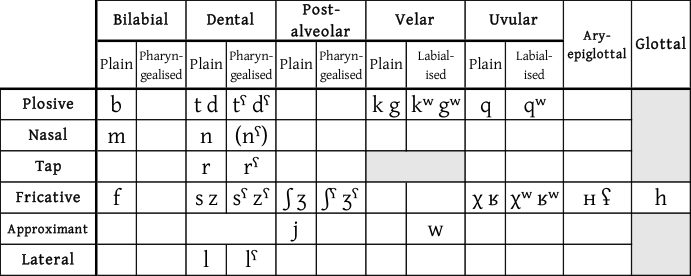
\includegraphics[width=1\textwidth]{figures/Table_3_1.png}
\caption{Consonant inventory of Tashlhiyt Berber, ignoring the singleton/geminate contrast (cf. \citealt{Ridouane2014}).}
   \label{tab:consonants}
   \end{table}

   
Tashlhiyt has a complex consonant system (see \tabref{tab:consonants}). Each singleton consonantal phoneme has a geminate counterpart. For example, consider the minimal pairs /juf/ ‘he was better’ vs. /juff/ ‘he puffed’ and /igwra/ ‘frogs’ vs. /iggwra/ ‘he was the last’. This length contrast is not restricted to word-medial position. It is also found in absolute initial and final positions.

Tashlhiyt contrasts plain and labialised dorsal consonants and plain and pharyngealised coronal consonants. Pharyngealisation, where it occurs, spreads towards adjacent segments. For example, in /tzdˤart/ ‘you are able’, the pharyngealisation of /dˤ/ spreads throughout the word (cf. \citealt{Ridouane2003}). The domain on which pharyngealisation operates has been identified as minimally the syllable and maximally the phonological word (\citealt{Elmedlaoui1995,DE2002}).

Tashlhiyt has two approximants, /j/ and /w/, which contrast with the corresponding high vowels /i, u/. Tashlhiyt has a rather simple vowel system with three lexical vowels /i, a, u/. The vowel quality has been reported to be highly dependent on the consonantal environment, especially regarding the presence or absence of adjacent pharyngealised consonants. As opposed to the consonantal system, vowels do not contrast with regard to length, although surface long vowels may occur in case of adjacent identical vowels. Any discussion of the Tashlhiyt vowel system should additionally refer to the existence of a central vowel that is not one of the cardinal vowels. The occurrence and distribution of this central vowel, often referred to as ‘schwa’, has sparked an as of yet unresolved debate as to whether this element needs to be considered as a phonological entity or a phonetic artefact (e.g. \citealt{Coleman1996,Coleman1999,Coleman2001,DE2002,Ridouane2008}, see Chapter 6 for a detailed discussion). This element is particularly relevant for the discussion of phonotactics and syllable structure, which we will turn to now.

\subsubsection{Phonotactics and syllable structure}
Tashlhiyt allows for whole utterances without any phonological vowels and has many words that consist of consonants only. Typologically rather rare structures such as \REF{ex:3:1} are often cited in the literature as extreme phonotactic cases. 

\begin{exe}
\ex\label{ex:3:1}   /tfttʃtsskkχtkkstʃʃkk/ \newline
‘You examined the currency which you checked out’ 
\end{exe}

Throughout this book, Tashlhiyt’s syllable structure will be described according to Dell and Elmedlaoui’s analyses (\citealt{DE1985,DE1988,DE1996,DE2002}) which is mainly based on the Imdlawn variety spoken by Elmedlaoui himself and, therefore, may be argued to have a limited generalisability. Even though we follow their analysis here, controversial aspects will be discussed where relevant. 

In addition to typologically common syllables containing vocalic nuclei such as V, CV, VC, and CVC, Tashlhiyt also has consonant-only syllables. According to Dell and Elmedlaoui, all consonant types are allowed in syllable nucleus position, even voiceless stops. This is exemplified in (\ref{ex:3:2}--\ref{ex:3:5}). 

\begin{exe}
\ex\label{ex:3:2}   Sonorants: /tl̩.km̩t/	‘You arrived’
\ex\label{ex:3:3} 	  Fricatives: /ts̩.χf̩t/ ‘You fainted’
\ex\label{ex:3:4}   Voiced stops: /tb̩.dg̍t/ ‘You are wet’
\ex\label{ex:3:5} 	  Voiceless stops: /tf̩.tk̩t/ ‘She sprained it’
\end{exe}

\subsection{Morphology}\label{sec:3.4.3}
The following brief sketch of morphological patterns in Tashlhiyt is based on Dell and Elmedlaoui’s descriptions (\citealt{DE1988,DE2002}). Tashlhiyt exhibits two major lexical categories: nouns and verbs. There is also a small group of adjectives, largely derived from verbs. Additionally, there are functional elements like tense and aspect markers, negation markers, complementisers, and conjunctions.

In general, verbs agree with their subjects in person, gender (feminine, masculine), and number (singular, plural) through prefixation, suffixation or both. Adjectives agree with the noun they modify in gender and number. Verb stems alternate according to aspect and mood resulting in four different stems per lexical verb (perfective affirmative, perfective negative, aorist, imperative). Stem alternation involves vowel alternation (vowel quality or alternation with null) or gemination.

Nouns are inflected for gender, number, and ‘state’ (free, bound). The grammatical category referred to as state (état d’annexion) has certain properties akin to case, e.g. it is dependent on the verbal and prepositional context. A noun is inflected for ‘bound state’ when it is governed by a preposition, when it follows its verb or a cardinal number. In all other positions, it is in the ‘free state’. However, not all nouns inflect for state. A distinction must be made between vowel-initial nouns (such as /agru/ ‘frog’) and consonant-initial nouns (such as /ssuq/ ‘market’). Consonant-initial nouns do not inflect for state, while vowel-initial nouns do. Gender and state are expressed through affixation, while number is expressed through either affixation or stem alternation. While affixation is regular, stem alternation is to some extent lexically determined. 

\subsection{Syntax}\label{sec:3.4.4}
The basic word order in Berber has been described as VSO (\citealt{Basset1952,Sasse1984}). Tashlhiyt is no exception, as can be seen in thetic utterances and most subordinate clauses (cf. \ref{ex:3:6}--\ref{ex:3:8} taken from \citealt[17]{DE2002}). All verbal arguments can be pronominalised. Referential pronouns are cliticised onto the verb (cf. \ref{ex:3:7}):

\ea\label{ex:3:6} 
\gll  t-ga t-fruχ-t i-fullus-n ʁ=t-gmmi \\
      \textsc{3f.sg}-put \textsc{f}-child.\textsc{bs-f.sg} up-chicken-\textsc{m.pl} in=\textsc{f}-house \\
\glt ‘The girl put the chickens into the house.’
\z

\ea\label{ex:3:7} 
\gll  t-ga=tn=gi-s \\
      \textsc{3f.sg}-put=\textsc{3m.pl}=in-\textsc{3f.sg} \\
\glt ‘She put them (m) into it (f).’
\z

The verb can carry cliticised pronouns for subject, indirect and direct object, multiple adverbs, and multiple prepositional phrases (in that order). If there is a clitic preponed to the verb, the pronouns cliticise to the preverb. In natural discourse, some verbal arguments are often contextually given and therefore pronominalised, in other contexts they are new information and expressed as full noun phrases. Most commonly, the subject is only expressed via a pronoun cliticised to the verb and the complements of the verb are expressed as full noun phrases (cf. \ref{ex:3:8}).

\ea\label{ex:3:8} 
\gll  t-ga i-fullus-n	ʁ=t-gmmi \\
      \textsc{3f.sg}-put up-chicken-\textsc{m.pl} in=\textsc{f}-house \\
\glt ‘She put the chickens into the house.’
\z

In the case of subject and direct object being expressed as proper noun phrases, SVO is also very common. When the subject precedes the verb, it is inflected for free state (cf. \ref{ex:3:9}).

\ea\label{ex:3:9} 
\gll  t-afruχ-t t-ga i-fullus-n ʁ=t-gm \\
      \textsc{f}-child-\textsc{f.sg} \textsc{3f.sg}-put up-chicken-\textsc{m.pl} in=\textsc{f}-house\\
\glt ‘The girl put the chickens into the house.’
\z

Both SVO and VSO are commonly used in cases of broad focus, i.e. as an answer to a question like /ma iʒran/ ‘what happened (or happens)?’. SVO constructions, however, are considered as carrying more emphasis (\citealt{Sadiqi1997,MettouchiFleisch2010}). This is particularly prominent in constructions having free standing pronouns (co-referential with the pronominal subject marker on the verb). These constructions appear to express emphasis if they are in clause-initial position (cf. \citealt[221]{MettouchiFleisch2010}). Other arguments of the verb can be left dislocated, too. Constructions with the subject or complements in clause-initial position are referred to as ‘left-dislocations’. In addition to left-dislocations, there are ‘cleft’ constructions. In cleft constructions, the subject or a complement of the verb occurs in clause-initial position preceding the verb. It is morphologically marked by a cleft marker (/ad/ cf. \ref{ex:3:10}).

\ea\label{ex:3:10} 
\gll  ddisk ad t-sʁa	t-fruχ-t  \\
      record ad \textsc{3f.sg}-bought \textsc{f}-child.\textsc{bs-f.sg} \\
\glt ‘It is a record that the girl bought.’
\z

Left-dislocated and clefted constituents are described as carrying pragmatic emphasis and have been reported to be prosodically separated from the rest of the utterance. \citet{MettouchiFleisch2010} note that in cleft constructions, the clefted constituent is separated from the verb by a “prosodic rupture” (ibid.: 224). On a similar note, Dell and Elmedlaoui speak of an “intonational break” (\citealt[17]{DE2002}) between the subject and the rest of the sentence in SVO constructions (see also \citealt{Shlonsky1987,Sadiqi1997,Boukhris.etal2008}).

Despite these impressionistic observations, higher prosodic aspects like stress and intonation are not yet systematically explored in Tashlhiyt. However, it is of particular relevance for intonation theory for two reasons: first, Tashlhiyt is renowned for cross-linguistically rare phonotactic flexibility, allowing whole utterances to consist of voiceless obstruents. This leads to frequent contexts in which the phonetic opportunity to execute pitch movements is drastically limited. The question arises as to how the language resolves this tune-text-association conflict. Second, impressionistic observations of different scholars throughout the last century have indicated that Tashlhiyt lacks word stress. The absence of lexically determined metrical structure raises the question as to how intonational tones are associated with segments. 
The question of whether Tashlhiyt exhibits word prosodic metrical structure, will be discussed in the following chapter.

